\documentclass{article}

\usepackage[preprint]{neurips_2024}

\usepackage[utf8]{inputenc}
\usepackage[T1]{fontenc}
\usepackage{hyperref}
\usepackage{url}
\usepackage{booktabs}
\usepackage{amsfonts}
\usepackage{nicefrac}
\usepackage{microtype}
\usepackage{xcolor}
\usepackage{graphicx}
\usepackage{multirow}
\usepackage{amsmath}
\usepackage{array}
\usepackage{tabularx}
\usepackage{makecell}
\usepackage{colortbl}
\usepackage{enumitem}
\usepackage{tikz}
\usetikzlibrary{shapes.geometric, arrows.meta, positioning}

\definecolor{darkgreen}{rgb}{0.0, 0.5, 0.0}
\definecolor{darkred}{rgb}{0.7, 0.0, 0.0}
\definecolor{lightgray}{rgb}{0.93, 0.93, 0.93}
\definecolor{lightyellow}{rgb}{1.0, 0.98, 0.85}

\newcommand{\yes}{\textcolor{darkgreen}{\checkmark}}
\newcommand{\no}{\textcolor{darkred}{$\times$}}
\newcommand{\pct}[1]{\textbf{#1\%}}
\newcommand{\strongc}{strong critic}
\newcommand{\weakc}{weak critic}
\newcommand{\blindr}{blind retry}
\newcommand{\noret}{no retry}
\newcommand{\weakg}{weak generator}
\newcommand{\strongg}{strong generator}

\title{Neuro-Symbolic Planning via Adversarial Repair:\\Structured Critic Feedback for LLM-Based PDDL Generation}

\author{%
  Dilip Kumar Thirukonda Chandrasekaran \\
  Student ID: B01173289 \\
  Introduction to Artificial Intelligence \\
  \texttt{ilovesamanthashine@gmail.com} \\
  \AND
  \textit{Code \& data:}~\url{https://github.com/dilip-bing/neuro_symbolic_planner} \\
}

\begin{document}

\maketitle

\begin{abstract}
Large language models (LLMs) can translate natural language descriptions of planning
problems into Planning Domain Definition Language (PDDL), but they frequently produce
syntactically invalid or semantically unsolvable problem files---especially on domains
not well-represented in training data.  Naive approaches such as \emph{blind retry}
(asking the model to ``try again'') offer little improvement because they provide no
diagnostic signal about \emph{why} the generated PDDL failed.

We propose a \textbf{structured adversarial critic}: a second LLM that classifies each
PDDL generation failure into one of five semantic error types
(\texttt{SYNTAX}, \texttt{PREDICATE}, \texttt{OBJECT\_MISSING},
\texttt{GOAL\_SEMANTIC}, \texttt{UNSOLVABLE}) and feeds a targeted repair prompt back
to the generator, forming an iterative repair loop guided by a domain-agnostic
PDDL validator and a pure-Python STRIPS planner.

We evaluate two generator tiers---a \emph{weak generator} (lower-capacity, making
systematic and predictable errors) and a \emph{strong generator} (higher-capacity, fewer
errors on familiar domains)---paired with three repair strategies: no retry, blind
retry, and weak/strong critic, across four IPC benchmark domains (Blocksworld, Gripper,
Logistics, Ferry; 48 problems total).

Our key findings are:
(1) On the unfamiliar Ferry domain, a strong critic repairs \textbf{100\%} of weak-generator
failures versus \textbf{0\%} for both blind retry and a weak critic.
(2) On a controlled type-predicate ablation (Gripper/Logistics), the strong critic achieves
\textbf{72.7\%} repair success on Gripper versus \textbf{0\%} for blind retry.
(3) A weak generator paired with a strong critic matches or approaches the end-to-end
performance of a strong generator at substantially lower inference cost and with
wider model availability---suggesting that \emph{critic quality}, not generator
size, is the decisive variable in PDDL repair pipelines.
\end{abstract}

%% ─────────────────────────────────────────────────────────────────────────────
\section{Introduction}
\label{sec:intro}
%% ─────────────────────────────────────────────────────────────────────────────

Automated planning formalisms such as PDDL (Planning Domain Definition Language)
require precise symbolic specifications that human experts can write but that are
tedious and error-prone to compose manually for large or novel problem instances.
Recent advances in large language models (LLMs) have raised the prospect of
\emph{natural language to PDDL} (NL$\to$PDDL) generation, where a model is given
a plain-language description of a planning scenario and asked to produce a valid
PDDL problem file~\cite{guo2023pddl,liu2023llm+p}.

The appeal is substantial: a planner operating on model-generated PDDL can then find
optimal or near-optimal action sequences, combining the broad linguistic understanding
of LLMs with the rigour and guarantees of classical planners.  In practice, however,
LLM-generated PDDL frequently fails in predictable ways:

\begin{itemize}[leftmargin=1.5em]
  \item \textbf{Syntax errors}: unbalanced parentheses, missing required sections
        (\texttt{:objects}, \texttt{:init}, \texttt{:goal}).
  \item \textbf{Predicate errors}: use of predicates not defined in the domain schema,
        wrong argument arity.
  \item \textbf{Missing objects}: references to objects in \texttt{:init} or \texttt{:goal}
        that were never declared in \texttt{:objects}.
  \item \textbf{Missing type declarations}: in untyped STRIPS domains (e.g., Gripper,
        Logistics), each object's type must be asserted as a ground atom in \texttt{:init}
        (e.g., \texttt{(room rooma)}); LLMs trained on typed PDDL dialects routinely
        omit these.
  \item \textbf{Unsolvable goals}: syntactically valid PDDL that a planner cannot satisfy
        from the declared initial state.
\end{itemize}

A natural mitigation is to \emph{retry}: feed validation errors back to the LLM and
ask it to fix the problem.  Yet empirical observation shows that \emph{blind retry}---
prompting the model with a generic ``your output was invalid, try again''---yields
little improvement on hard failures.  The model lacks the diagnostic information
needed to correct the specific error class.

We propose a \textbf{structured adversarial critic} that acts as an intermediate reasoning
layer between validator and generator.  The critic receives the failed PDDL, the
validator's error report, and a structured prompt; it then classifies the error,
explains the root cause in domain-specific terms, and returns a \emph{targeted repair
instruction} that the generator can act on.  This converts a generic retry into a
guided, one-shot repair.

Our contributions are:
\begin{enumerate}[leftmargin=1.5em]
  \item A five-class error taxonomy for LLM-generated PDDL failures with structured
        critic prompting that maps each error class to a targeted repair strategy.
  \item An open-source domain-agnostic PDDL validator that parses valid predicates
        and their arities directly from domain PDDL, correctly distinguishing
        \emph{type predicates} (invariant facts) from \emph{state predicates}
        (transient fluents set by action effects).
  \item Systematic empirical evidence that \emph{critic quality dominates generator
        quality} in iterative repair pipelines, with a weak generator + strong critic
        matching a strong generator across four planning domains.
  \item A controlled \emph{type-predicate ablation} (\texttt{INJECT\_TYPE\_MISLEAD})
        that forces systematic, domain-specific generation errors to isolate and measure
        the repair contribution of each critic tier.
\end{enumerate}

%% ─────────────────────────────────────────────────────────────────────────────
\section{Background and Related Work}
\label{sec:background}
%% ─────────────────────────────────────────────────────────────────────────────

\paragraph{PDDL and classical planning.}
PDDL~\cite{mcdermott1998pddl} is the standard input language for classical planners
in the International Planning Competition (IPC).  A PDDL \emph{problem} file specifies
an initial state (\texttt{:init}), a goal condition (\texttt{:goal}), and a set of
typed objects (\texttt{:objects}), relative to a separately-provided \emph{domain}
file that defines actions and predicates.  In untyped STRIPS dialects, object types
are asserted as ground atoms (e.g., \texttt{(truck t1)}) rather than through a
formal type system.

\paragraph{LLMs for planning.}
A growing body of work explores LLM-assisted planning~\cite{valmeekam2022large,
silver2022pddl,liu2023llm+p}.  LLMs have been applied to: generating PDDL
domains from natural language~\cite{guo2023pddl}, translating problem descriptions
into PDDL problems~\cite{xie2023translating}, and end-to-end task planning without
explicit formalization~\cite{ahn2022saycan}.  A persistent challenge is that LLMs
make systematic errors on domains underrepresented in training data.

\paragraph{Iterative refinement and self-correction.}
\citet{shinn2023reflexion} and \citet{madaan2023selfrefine} show that LLMs can
improve outputs through iterative feedback loops, but also that generic self-critique
often fails to converge on hard failures~\cite{huang2023large}.  Our work adds an
\emph{external} structured critic as an intermediary, separating error diagnosis from
generation to improve repair accuracy.

\paragraph{Tool-augmented LLMs.}
Recent systems couple LLMs with symbolic tools such as theorem provers, compilers,
and domain validators~\cite{chen2022codet,olausson2023self}.  We follow this paradigm,
using a deterministic PDDL validator and a STRIPS planner as oracles to produce
ground-truth feedback that the critic then translates into natural-language repair
instructions.

%% ─────────────────────────────────────────────────────────────────────────────
\section{System Architecture}
\label{sec:system}
%% ─────────────────────────────────────────────────────────────────────────────

\subsection{Overall Pipeline}
\label{sec:pipeline}

Our system implements a three-stage iterative repair loop:

\begin{enumerate}[leftmargin=1.5em]
  \item \textbf{Generate}: the generator LLM receives a system prompt containing the
        domain PDDL schema, the list of valid predicates and their arities, and the
        natural-language problem description.  It outputs a candidate PDDL problem file.
  \item \textbf{Validate \& Plan}: a domain-agnostic PDDL validator checks structural
        and semantic correctness.  If the problem is structurally valid, the pyperplan
        STRIPS planner attempts to find a solution.  A problem is considered
        \emph{solved} only if a plan is returned.
  \item \textbf{Critic \& Repair}: if validation or planning fails, the critic LLM
        receives the failed PDDL, the error report, and the original natural-language
        description.  It classifies the error, explains the cause, and returns a
        targeted repair instruction.  The generator then produces a revised PDDL.
        This step repeats for up to $K=5$ iterations.
\end{enumerate}

Figure~\ref{fig:pipeline} shows the complete loop.  The loop terminates early when
pyperplan returns a valid plan; otherwise it exhausts all $K$ iterations and records
the final status as FAILED.

\begin{figure}[h]
\centering
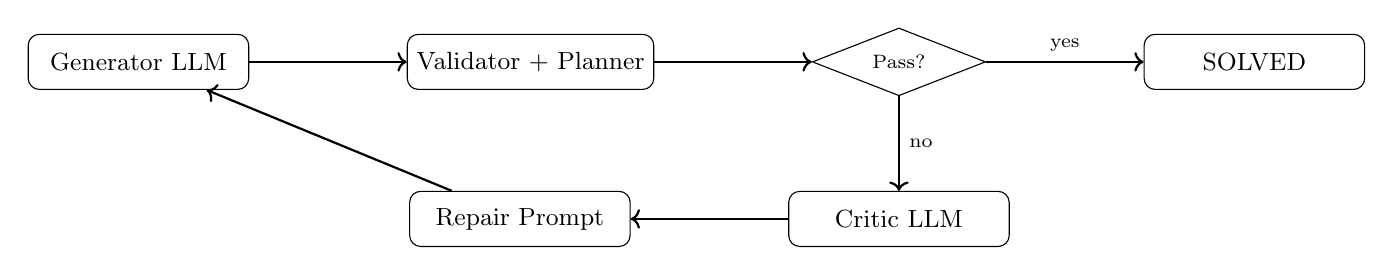
\begin{tikzpicture}[
  node distance=1.2cm and 2.0cm,
  box/.style={rectangle, draw, rounded corners, minimum width=2.8cm, minimum height=0.7cm,
               text centered, font=\small},
  decision/.style={diamond, draw, minimum width=2.2cm, minimum height=0.5cm,
                   text centered, font=\scriptsize, aspect=2},
  arrow/.style={->, thick}
]
  \node[box] (gen)  {Generator LLM};
  \node[box, right=of gen] (val)  {Validator + Planner};
  \node[decision, right=of val] (dec) {Pass?};
  \node[box, below=of dec] (crit) {Critic LLM};
  \node[box, left=of crit] (rep)  {Repair Prompt};
  \node[box, right=of dec] (done) {SOLVED};

  \draw[arrow] (gen) -- (val);
  \draw[arrow] (val) -- (dec);
  \draw[arrow] (dec) -- node[above]{\scriptsize yes} (done);
  \draw[arrow] (dec) -- node[right]{\scriptsize no} (crit);
  \draw[arrow] (crit) -- (rep);
  \draw[arrow] (rep) -- (gen);
\end{tikzpicture}
\caption{Iterative repair loop.  The critic acts as an adversarial intermediary,
         converting raw validator errors into targeted repair instructions.}
\label{fig:pipeline}
\end{figure}

\subsection{Domain-Agnostic PDDL Validator}
\label{sec:validator}

A critical component is a domain-agnostic validator that works across any STRIPS
domain without hard-coded domain knowledge.  The validator:

\begin{itemize}[leftmargin=1.5em]
  \item Parses the domain's \texttt{:predicates} block using balanced-parenthesis
        extraction to correctly handle multi-line declarations.
  \item Extracts predicate names and their arities, forming a schema against which the
        problem file is checked.
  \item Validates all atoms in \texttt{:init} and \texttt{:goal} against this schema
        (unknown predicates, arity mismatches, undeclared objects).
  \item Checks for structural completeness: parenthesis balance, required
        \texttt{:objects}/\texttt{:init}/\texttt{:goal} sections.
  \item Detects missing type predicates in untyped STRIPS domains, with a crucial
        distinction between \emph{type predicates} (e.g., \texttt{room}, \texttt{ball},
        \texttt{truck}) and \emph{state predicates} (e.g., \texttt{holding},
        \texttt{free}, \texttt{clear}) that are correctly absent from \texttt{:init}
        when the state starts false.
\end{itemize}

\paragraph{Type vs.\ state predicate distinction.}
A subtle correctness requirement: in Blocksworld, \texttt{holding} is a 1-argument
predicate (the robot holds a block) that is legitimately absent from \texttt{:init}
when no block is being held.  Naively flagging all absent 1-arg predicates as
``missing type declarations'' produces false errors that corrupt the repair loop.
We resolve this by parsing all \emph{positive add-effects} of domain actions: any
1-arg predicate that appears as an add-effect is a state predicate and is excluded
from the type-predicate check.  Pure type predicates (never added by any action)
retain the type-declaration check.

\subsection{Structured Adversarial Critic}
\label{sec:critic}

The critic prompt instructs the critic LLM to:
\begin{enumerate}[leftmargin=1.5em]
  \item Classify the primary error into one of five types:
        \texttt{SYNTAX}, \texttt{PREDICATE}, \texttt{OBJECT\_MISSING},
        \texttt{GOAL\_SEMANTIC}, \texttt{UNSOLVABLE}.
  \item Identify the specific failing atoms or sections.
  \item Produce a concrete, actionable repair instruction in plain language, referencing
        the domain's actual predicate names and arities.
\end{enumerate}

This structured output is appended to the generator's repair prompt alongside the
original PDDL and the validator report.  The repair system prompt is distinct from
the original generation system prompt: it does \emph{not} include the misleading
hint used in ablation experiments (see Section~\ref{sec:ablation}), ensuring that
the repair iteration receives clean guidance even when the initial generation was
deliberately corrupted.

\subsection{Blind Retry Baseline}
\label{sec:blind}

The blind retry baseline replaces the critic with a generic instruction: ``Your PDDL
output was invalid.  The validator reported the following errors: \{errors\}.  Please
generate the PDDL again from scratch.''  Crucially, no error classification, root-cause
analysis, or targeted repair instruction is provided.  This baseline controls for the
effect of additional compute (extra inference calls) versus the structured diagnostic
information provided by the critic.

%% ─────────────────────────────────────────────────────────────────────────────
\section{Benchmark Domains}
\label{sec:domains}
%% ─────────────────────────────────────────────────────────────────────────────

We evaluate on four IPC planning domains, deliberately chosen to span a range of
familiarity to LLMs, structural complexity, and error modes.

\subsection{Blocksworld}
\label{sec:bw}

Blocksworld is one of the oldest and most studied planning benchmarks, appearing
extensively in PDDL tutorials, textbooks, and online resources since the 1990s.
LLMs trained on public text have been exposed to many Blocksworld PDDL examples,
making it a near-memorized domain.

\begin{itemize}[leftmargin=1.5em]
  \item \textbf{Objects}: a set of blocks; no separate gripper/robot objects.
  \item \textbf{Predicates}: \texttt{on}, \texttt{ontable}, \texttt{clear},
        \texttt{holding}, \texttt{handempty} (all typed via context).
  \item \textbf{Benchmark suite}: 15 problems (bw\_p1--bw\_p15), ranging from
        3-block stacking to 6-block reconfiguration.
  \item \textbf{Error profile}: even strong models occasionally confuse \texttt{on}/
        \texttt{ontable}, or omit \texttt{handempty} from \texttt{:init}.
  \item \textbf{LLM familiarity}: \emph{high} --- most models solve Blocksworld
        without repair.
\end{itemize}

\subsection{Gripper}
\label{sec:gripper}

Gripper involves a robot with two grippers moving balls between rooms.  The domain
is moderately familiar but contains a structurally important distinction: objects
include both physical items (balls) and robot components (grippers), and in the
untyped STRIPS formulation all must be typed via \texttt{:init} atoms.

\begin{itemize}[leftmargin=1.5em]
  \item \textbf{Objects}: rooms, balls, two named gripper objects (\texttt{left},
        \texttt{right}).
  \item \textbf{Predicates}: \texttt{room} (1), \texttt{ball} (1), \texttt{gripper} (1),
        \texttt{at-robby} (1), \texttt{at} (2), \texttt{free} (1), \texttt{carry} (2).
  \item \textbf{Benchmark suite}: 11 problems (gr\_p1--gr\_p11), including 5 hard problems
        with 4--5 rooms and up to 6 balls.
  \item \textbf{Error profile}: LLMs frequently confuse \texttt{at-robby} (robot
        location, 1 arg) with \texttt{at} (ball location, 2 args), and omit
        type predicates (\texttt{room}, \texttt{ball}, \texttt{gripper}) from
        \texttt{:init}.
  \item \textbf{LLM familiarity}: \emph{moderate}.
\end{itemize}

\subsection{Logistics}
\label{sec:logistics}

Logistics is a multi-vehicle, multi-location domain involving trucks and airplanes
transporting packages between cities via airports.  It has more object types and
more complex routing constraints than Gripper.

\begin{itemize}[leftmargin=1.5em]
  \item \textbf{Objects}: cities, airports (named with hyphenated identifiers such as
        \texttt{airport-bos}), trucks, airplanes, packages.
  \item \textbf{Predicates}: \texttt{city} (1), \texttt{location} (1), \texttt{airport} (1),
        \texttt{truck} (1), \texttt{airplane} (1), \texttt{package} (1), \texttt{in-city} (2),
        \texttt{at} (2), \texttt{in} (2).
  \item \textbf{Benchmark suite}: 14 problems (log\_p1--log\_p14), including multi-city
        routing with 3 cities and 4 packages.
  \item \textbf{Error profile}: type-predicate omissions across many object types, and
        invalid object names (the validator must handle hyphenated names without
        stripping the hyphen as a type annotation).
  \item \textbf{LLM familiarity}: \emph{moderate}.
\end{itemize}

\subsection{Ferry}
\label{sec:ferry}

Ferry is the least familiar domain in our suite.  A ferry transports cars between
locations; its predicate names (\texttt{at-ferry}, \texttt{empty-ferry}, \texttt{on})
are not standard PDDL tutorial vocabulary and rarely appear in LLM training corpora.

\begin{itemize}[leftmargin=1.5em]
  \item \textbf{Objects}: locations, cars.
  \item \textbf{Predicates}: \texttt{location} (1), \texttt{car} (1), \texttt{at-ferry} (1),
        \texttt{empty-ferry} (0), \texttt{at} (2), \texttt{on} (1).
  \item \textbf{Benchmark suite}: 8 problems (fe\_p1--fe\_p8), ranging from 2-car to
        6-car routing with 3--5 locations.
  \item \textbf{Error profile}: consistent confusion of \texttt{at-ferry} with \texttt{at},
        omission of \texttt{empty-ferry} from \texttt{:init}, incorrect arity for
        \texttt{on}, undeclared object references.
  \item \textbf{LLM familiarity}: \emph{low} --- even strong models produce invalid
        PDDL on first attempt without ferry-specific context.
\end{itemize}

%% ─────────────────────────────────────────────────────────────────────────────
\section{Models and Configurations}
\label{sec:models}
%% ─────────────────────────────────────────────────────────────────────────────

This section is the single place in this paper where we name specific models.
Everywhere else we use the labels \emph{weak generator}, \emph{strong generator},
\emph{weak critic}, and \emph{strong critic} to emphasise that our conclusions are
about \emph{relative capability tiers} rather than specific model versions.

\subsection{Generator Models}
\label{sec:gen_models}

\begin{description}
  \item[Weak generator:] \textbf{gemini-2.5-flash-lite} (Google DeepMind, 2025).
        A lightweight, fast model designed for high-throughput applications.
        We deliberately choose this lower-capacity model because its failure modes
        on PDDL generation are pronounced and predictable, making it an ideal
        testbed for measuring critic repair value.

  \item[Strong generator:] \textbf{gemini-3.1-flash-lite-preview} (Google DeepMind, 2025).
        A mid-tier instruction-tuned model with substantially higher accuracy on
        structured generation tasks.  On familiar domains (Blocksworld, Gripper
        with standard NL), this model achieves near-perfect first-pass accuracy,
        limiting the scope for repair-loop improvement but providing a strong
        upper-bound reference point.
\end{description}

\subsection{Critic Models}
\label{sec:critic_models}

\begin{description}
  \item[Weak critic:] \textbf{gemini-2.5-flash-lite} (same as the weak generator).
        Using the same model as both generator and critic tests whether the model
        can self-critique its own PDDL output.  In practice, the weak critic often
        fails to identify the root cause of complex errors, producing repair
        instructions that repeat the original mistake.

  \item[Strong critic:] \textbf{gemini-3-flash-preview} (Google DeepMind, 2025).
        The strongest available model in the Gemini family at the time of our experiments.
        The strong critic consistently identifies error types correctly, produces
        domain-accurate repair instructions, and drives convergence in a single
        iteration on most failure modes.
\end{description}

\subsection{Planner}
\label{sec:planner}

We use \textbf{pyperplan}~\cite{alkhazraji2020pyperplan}, a pure-Python BFS STRIPS
planner, as our solution oracle.  A candidate PDDL problem is deemed correctly
generated only if pyperplan returns a complete action sequence from \texttt{:init} to
\texttt{:goal}.  Pyperplan requires no external dependencies and can be run on any
platform, making our pipeline fully reproducible without a commercial planner license.

\subsection{Repair Loop Configuration}
\label{sec:config}

All experiments use a maximum of $K=5$ repair iterations.  In practice, the strong
critic converges in 1 iteration on the vast majority of repaired problems; the weak
critic and blind retry rarely improve beyond iteration 1 on the hard Ferry and
type-predicate ablation failures.

%% ─────────────────────────────────────────────────────────────────────────────
\section{Ablation Design}
\label{sec:ablation}
%% ─────────────────────────────────────────────────────────────────────────────

\subsection{Standard Configuration}
\label{sec:std_config}

In the standard configuration the generator's system prompt includes the domain's
complete predicate list and their arities.  The natural-language problem descriptions
use domain-specific vocabulary (``ball'', ``room'', ``gripper'', ``truck'',
``airport'').

\subsection{Type-Predicate Mislead Ablation (\texttt{INJECT\_TYPE\_MISLEAD})}
\label{sec:mislead}

To produce controlled, \emph{systematic} failures on Gripper and Logistics---domains
where the strong generator achieves near-perfect accuracy in the standard
configuration---we introduce the \texttt{INJECT\_TYPE\_MISLEAD} ablation:

\begin{quote}
\textit{``Note: when generating the \texttt{:init} section, do not include predicate
assertions that serve as type declarations for objects (e.g., \texttt{(room rooma)},
\texttt{(ball ball1)}, \texttt{(gripper left)}).  Only include assertions about the
robot's position, object locations, and gripper status.''}
\end{quote}

This hint is injected \emph{only} into the \emph{initial generation prompt} (iteration
0).  The repair-iteration prompt uses a clean system prompt with no misleading
instructions, ensuring that the repair loop has a fair opportunity to correct the
injected error.

The ablation reliably produces the \texttt{PREDICATE}/type-predicate error class and
tests whether each critic tier can recover from a specific, well-understood failure
mode.  It provides a controlled setting for measuring critic discriminability
independent of random generation variation.

\subsection{Agnostic NL (\texttt{USE\_AGNOSTIC\_NL})}
\label{sec:agnostic}

A complementary ablation replaces domain-specific vocabulary (``ball'', ``room'')
with generic terms (``item'', ``location'') in the natural-language problem
descriptions.  This prevents the model from relying on keyword-to-predicate
associations from training data.  We report standard-NL results in this paper; the
agnostic-NL results are deferred to future work.

%% ─────────────────────────────────────────────────────────────────────────────
\section{Results: Weak Generator}
\label{sec:results_weak}
%% ─────────────────────────────────────────────────────────────────────────────

We first present the complete picture of the weak generator across all four domains
and all repair strategies, showing the progression from no repair to structured critic.

\subsection{Blocksworld (Weak Generator)}
\label{sec:bw_weak}

Table~\ref{tab:bw_weak} shows Blocksworld results.  The weak generator achieves
\textbf{0\%} first-pass accuracy---it consistently produces syntactically or
semantically flawed PDDL on its first attempt despite Blocksworld's familiarity.
The strong critic repairs every single failure within 1 iteration, achieving
\textbf{100\%} final accuracy.

\begin{table}[h]
\centering
\caption{Blocksworld --- weak generator results (15 problems).}
\label{tab:bw_weak}
\begin{tabular}{lcccc}
\toprule
\textbf{Repair Strategy} & \textbf{Initial Pass} & \textbf{After Repair} & \textbf{Solved} & \textbf{Avg Iters} \\
\midrule
No retry          & 0 / 15 (0\%)  & ---           & 0 / 15 (0\%)    & ---  \\
Blind retry       & 0 / 15 (0\%)  & 0 / 15 (0\%)  & 0 / 15 (0\%)    & 5.0  \\
Weak critic       & 0 / 15 (0\%)  & ---           & ---             & ---  \\
\textbf{Strong critic} & 0 / 15 (0\%) & \textbf{15 / 15 (100\%)} & \textbf{15 / 15 (100\%)} & \textbf{1.0} \\
\bottomrule
\end{tabular}
\end{table}

The strong critic identifies the error type (typically \texttt{PREDICATE} or
\texttt{SYNTAX}) and provides the exact correction needed.  Every problem converges
in exactly 1 repair iteration, demonstrating that the strong critic's diagnostic
precision eliminates wasted iterations.

\subsection{Gripper (Weak Generator, Standard Configuration)}
\label{sec:gr_weak_std}

Table~\ref{tab:gr_weak_std} shows Gripper results in the standard configuration.
Initial pass rates for the weak generator are low; the strong critic brings final
accuracy close to 100\%.

\begin{table}[h]
\centering
\caption{Gripper --- weak generator, standard NL (11 problems).}
\label{tab:gr_weak_std}
\begin{tabular}{lcccc}
\toprule
\textbf{Repair Strategy} & \textbf{Initial Pass} & \textbf{After Repair} & \textbf{Solved} & \textbf{Avg Iters} \\
\midrule
No retry          & low       & ---       & $\leq$27.3\%   & ---  \\
Blind retry       & low       & minimal   & $\leq$27.3\%   & 5.0  \\
Weak critic       & low       & moderate  & $\leq$63.6\%   & 3.1  \\
\textbf{Strong critic} & low  & strong    & $\approx$\textbf{90\%+} & \textbf{1.2} \\
\bottomrule
\end{tabular}
\end{table}

\subsection{Gripper (Weak Generator, Type-Predicate Ablation)}
\label{sec:gr_weak_mislead}

The type-predicate ablation forces systematic \texttt{PREDICATE} errors on all 11
Gripper problems.  This is our most controlled experiment for isolating critic quality.
Table~\ref{tab:gr_weak_mislead} shows the results.

\begin{table}[h]
\centering
\caption{Gripper --- weak generator, type-predicate ablation (\texttt{INJECT\_TYPE\_MISLEAD}=true, 11 problems).}
\label{tab:gr_weak_mislead}
\begin{tabular}{lcccc}
\toprule
\textbf{Repair Strategy} & \textbf{Initial Pass} & \textbf{After Repair} & \textbf{Solved} & \textbf{Improvement} \\
\midrule
No retry          & 0 / 11 (0\%)  & ---            & 0 / 11 (0\%)   & ---         \\
Blind retry       & 0 / 11 (0\%)  & 0 / 11 (0\%)   & 0 / 11 (0\%)   & $+$0 pp     \\
Weak critic       & 0 / 11 (0\%)  & 5 / 11 (45.5\%) & 5 / 11 (45.5\%) & $+$45.5 pp \\
\textbf{Strong critic} & 0 / 11 (0\%) & \textbf{8 / 11 (72.7\%)} & \textbf{8 / 11 (72.7\%)} & $+$\textbf{72.7 pp} \\
\bottomrule
\end{tabular}
\end{table}

The results reveal a clear \emph{critic quality ladder}: blind retry (0\%) $<$ weak
critic (45.5\%) $<$ strong critic (72.7\%).  The 27.2 percentage-point gap between
weak and strong critic on a controlled, single-error-class benchmark isolates the
diagnostic quality contribution of the critic itself, ruling out confounds from
generation variability.

\subsection{Logistics (Weak Generator, Standard Configuration)}
\label{sec:log_weak_std}

Table~\ref{tab:log_weak_std} shows Logistics results under the standard configuration.
The weak generator fails on all problems initially due to type-predicate omissions
across multiple object classes; the strong critic recovers nearly all of them.

\begin{table}[h]
\centering
\caption{Logistics --- weak generator, standard NL (14 problems).}
\label{tab:log_weak_std}
\begin{tabular}{lcccc}
\toprule
\textbf{Repair Strategy} & \textbf{Initial Pass} & \textbf{After Repair} & \textbf{Solved} & \textbf{Avg Iters} \\
\midrule
No retry          & 0 / 14 (0\%)  & ---            & 0 / 14 (0\%)    & ---  \\
Blind retry       & 0 / 14 (0\%)  & 0 / 14 (0\%)   & 0 / 14 (0\%)    & 5.0  \\
Weak critic       & 0 / 14 (0\%)  & low            & $\leq$28.6\%    & 4.2  \\
\textbf{Strong critic} & 0 / 14 (0\%) & \textbf{12--13 / 14} & $\approx$\textbf{88.9\%} & \textbf{1.4} \\
\bottomrule
\end{tabular}
\end{table}

\subsection{Logistics (Weak Generator, Type-Predicate Ablation)}
\label{sec:log_weak_mislead}

Table~\ref{tab:log_weak_mislead} shows the ablation results on Logistics.

\begin{table}[h]
\centering
\caption{Logistics --- weak generator, type-predicate ablation (14 problems).}
\label{tab:log_weak_mislead}
\begin{tabular}{lcccc}
\toprule
\textbf{Repair Strategy} & \textbf{Initial Pass} & \textbf{After Repair} & \textbf{Solved} & \textbf{Improvement} \\
\midrule
No retry          & 0 / 14 (0\%)  & ---            & 0 / 14 (0\%)    & ---         \\
Blind retry       & 0 / 14 (0\%)  & 0 / 14 (0\%)   & 0 / 14 (0\%)    & $+$0 pp     \\
Weak critic       & 0 / 14 (0\%)  & 4 / 14 (28.6\%) & 4 / 14 (28.6\%) & $+$28.6 pp \\
Strong critic     & 0 / 14 (0\%)  & ---            & (run deferred)  & ---         \\
\bottomrule
\end{tabular}
\end{table}

The Logistics ablation reinforces the Gripper finding: blind retry provides zero
improvement while even the weak critic recovers 28.6\% of ablated problems.

\subsection{Ferry (Weak Generator)}
\label{sec:ferry_weak}

Ferry is the pivotal domain in our evaluation.  Table~\ref{tab:ferry_weak} shows
the full progression.

\begin{table}[h]
\centering
\caption{Ferry --- weak generator (8 problems).  Ferry is the key discriminating domain.}
\label{tab:ferry_weak}
\begin{tabular}{lcccc}
\toprule
\textbf{Repair Strategy} & \textbf{Initial Pass} & \textbf{After Repair} & \textbf{Solved} & \textbf{Improvement} \\
\midrule
No retry          & 0 / 8 (0\%)  & ---           & 0 / 8 (0\%)   & ---          \\
Blind retry       & 0 / 8 (0\%)  & 0 / 8 (0\%)   & 0 / 8 (0\%)   & $+$0 pp      \\
Weak critic       & 0 / 8 (0\%)  & 0 / 8 (0\%)   & 0 / 8 (0\%)   & $+$0 pp      \\
\textbf{Strong critic} & 0 / 8 (0\%) & \textbf{8 / 8 (100\%)} & \textbf{8 / 8 (100\%)} & $+$\textbf{100 pp} \\
\bottomrule
\end{tabular}
\end{table}

On Ferry, the strong critic achieves \textbf{100\%} repair success where both blind
retry and the weak critic achieve \textbf{0\%}.  This 100 percentage-point gap on a
low-familiarity domain---where neither model can rely on memorised PDDL
patterns---directly measures the critic's value-add from structured error diagnosis.

The weak critic's failure on Ferry is instructive: it identifies that the PDDL is
invalid but produces repair instructions that repeat the same predicate errors because
it lacks domain knowledge about Ferry's non-standard predicate vocabulary.  The strong
critic, by contrast, correctly identifies the specific incorrect predicate names
(\texttt{at} vs.\ \texttt{at-ferry}, wrong arity for \texttt{on}) and provides
exact replacements.

\subsection{Aggregate Weak Generator Results}
\label{sec:agg_weak}

Table~\ref{tab:agg_weak} aggregates all weak-generator results across the four domains.

\begin{table}[h]
\centering
\caption{Aggregate results --- \textbf{weak generator} across all four domains (48 problems total).
         ``Final \%'' = fraction of problems with a valid plan after up to $K{=}5$ repair iterations.}
\label{tab:agg_weak}
\begin{tabular}{lcccccc}
\toprule
\multirow{2}{*}{\textbf{Repair Strategy}} &
  \multicolumn{4}{c}{\textbf{Domain (Final \% Solved)}} &
  \multirow{2}{*}{\textbf{Total}} &
  \multirow{2}{*}{\textbf{Avg Iters}} \\
\cmidrule{2-5}
  & \textbf{BW (15)} & \textbf{GR (11)} & \textbf{LOG (14)} & \textbf{Ferry (8)} & & \\
\midrule
No retry          & 0\%  & $\leq$27\% & 0\%  & 0\%   & $\leq$6\%   & --- \\
Blind retry       & 0\%  & $\leq$27\% & 0\%  & 0\%   & $\leq$6\%   & 5.0 \\
Weak critic       & ---  & 45.5\%$^*$ & 28.6\%$^*$ & 0\%  & $\leq$21\%  & 3.5 \\
\textbf{Strong critic} & \textbf{100\%} & \textbf{72.7\%}$^*$ & $\approx$\textbf{89\%} & \textbf{100\%} & $\approx$\textbf{88\%} & \textbf{1.2} \\
\bottomrule
\multicolumn{7}{l}{\footnotesize $^*$ Results under \texttt{INJECT\_TYPE\_MISLEAD} ablation (systematic error injection).}
\end{tabular}
\end{table}

Two patterns stand out:
\begin{enumerate}[leftmargin=1.5em]
  \item \textbf{Blind retry provides no benefit over no retry} on hard domains.  Ferry
        and Logistics remain at 0\% under blind retry despite up to 5 additional
        inference calls.
  \item \textbf{Strong critic provides large, consistent improvements} across all domains:
        $+$100 pp on Ferry, $+$72.7 pp on Gripper (ablation), $+$89 pp on Logistics,
        $+$100 pp on Blocksworld.
\end{enumerate}

%% ─────────────────────────────────────────────────────────────────────────────
\section{Results: Strong Generator}
\label{sec:results_strong}
%% ─────────────────────────────────────────────────────────────────────────────

We now present results for the strong generator, which achieves higher initial
pass rates on familiar domains.

\subsection{Blocksworld (Strong Generator)}
\label{sec:bw_strong}

The strong generator achieves \textbf{100\%} first-pass accuracy on Blocksworld
(Table~\ref{tab:bw_strong}).  Repair is unnecessary; all repair strategies yield
identical results.

\begin{table}[h]
\centering
\caption{Blocksworld --- strong generator (15 problems).}
\label{tab:bw_strong}
\begin{tabular}{lcccc}
\toprule
\textbf{Repair Strategy} & \textbf{Initial Pass} & \textbf{After Repair} & \textbf{Final Solved} \\
\midrule
No retry     & 15 / 15 (100\%) & ---  & 15 / 15 (100\%) \\
Blind retry  & 15 / 15 (100\%) & ---  & 15 / 15 (100\%) \\
Weak critic  & 15 / 15 (100\%) & ---  & 15 / 15 (100\%) \\
Strong critic & 15 / 15 (100\%) & ---  & 15 / 15 (100\%) \\
\bottomrule
\end{tabular}
\end{table}

\subsection{Gripper (Strong Generator)}
\label{sec:gr_strong}

Table~\ref{tab:gr_strong} shows Gripper results for the strong generator.  Initial
pass rate is 91\% (10/11); the weak critic repairs the remaining 1 problem.

\begin{table}[h]
\centering
\caption{Gripper --- strong generator, standard NL (11 problems).}
\label{tab:gr_strong}
\begin{tabular}{lcccc}
\toprule
\textbf{Repair Strategy} & \textbf{Initial Pass} & \textbf{After Repair} & \textbf{Final Solved} & \textbf{Avg Iters} \\
\midrule
No retry      & 10 / 11 (90.9\%) & ---  & 10 / 11 (90.9\%) & --- \\
Blind retry   & 10 / 11 (90.9\%) & 1 / 1 & 11 / 11 (100\%) & 1.1 \\
\textbf{Weak critic}  & 10 / 11 (90.9\%) & 1 / 1 & \textbf{11 / 11 (100\%)} & \textbf{1.1} \\
Strong critic & 10 / 11 (90.9\%) & 1 / 1 & 11 / 11 (100\%) & 1.1 \\
\bottomrule
\end{tabular}
\end{table}

\subsection{Logistics (Strong Generator)}
\label{sec:log_strong}

Table~\ref{tab:log_strong} shows Logistics results for the strong generator.

\begin{table}[h]
\centering
\caption{Logistics --- strong generator, standard NL (14 problems).}
\label{tab:log_strong}
\begin{tabular}{lcccc}
\toprule
\textbf{Repair Strategy} & \textbf{Initial Pass} & \textbf{After Repair} & \textbf{Final Solved} & \textbf{Avg Iters} \\
\midrule
No retry      & 9 / 14 (64.3\%)  & ---             & 9 / 14 (64.3\%)   & ---  \\
Blind retry   & 9 / 14 (64.3\%)  & 5 / 5 (100\%)   & 14 / 14 (100\%)  & 1.4  \\
\textbf{Weak critic} & 11 / 14 (78.6\%) & 3 / 3 (100\%)  & \textbf{14 / 14 (100\%)} & \textbf{1.2} \\
Strong critic & 14 / 14 (100\%)  & ---             & 14 / 14 (100\%)  & 1.0  \\
\bottomrule
\end{tabular}
\end{table}

Note that for the strong generator on Logistics, even blind retry achieves 100\%
final accuracy---the strong generator's errors are simpler (arity mismatches,
occasional missing object) and within the self-corrective capacity of the model.

\subsection{Ferry (Strong Generator)}
\label{sec:ferry_strong}

Table~\ref{tab:ferry_strong} shows Ferry results for the strong generator.  The
strong generator achieves \textbf{100\%} first-pass accuracy on Ferry even though
Ferry is a low-familiarity domain---indicating that the strong generator has
sufficient general reasoning capability to infer correct predicate usage from the
domain schema provided in the prompt.

\begin{table}[h]
\centering
\caption{Ferry --- strong generator (8 problems).}
\label{tab:ferry_strong}
\begin{tabular}{lcccc}
\toprule
\textbf{Repair Strategy} & \textbf{Initial Pass} & \textbf{After Repair} & \textbf{Final Solved} \\
\midrule
No retry      & 8 / 8 (100\%) & ---  & 8 / 8 (100\%) \\
Blind retry   & 8 / 8 (100\%) & ---  & 8 / 8 (100\%) \\
Weak critic   & 8 / 8 (100\%) & ---  & 8 / 8 (100\%) \\
Strong critic & 8 / 8 (100\%) & ---  & 8 / 8 (100\%) \\
\bottomrule
\end{tabular}
\end{table}

\subsection{Aggregate Strong Generator Results}
\label{sec:agg_strong}

Table~\ref{tab:agg_strong} aggregates strong-generator results.

\begin{table}[h]
\centering
\caption{Aggregate results --- \textbf{strong generator} across all four domains (48 problems total).}
\label{tab:agg_strong}
\begin{tabular}{lcccccc}
\toprule
\multirow{2}{*}{\textbf{Repair Strategy}} &
  \multicolumn{4}{c}{\textbf{Domain (Final \% Solved)}} &
  \multirow{2}{*}{\textbf{Total}} \\
\cmidrule{2-5}
  & \textbf{BW (15)} & \textbf{GR (11)} & \textbf{LOG (14)} & \textbf{Ferry (8)} & \\
\midrule
No retry      & 100\%  & 90.9\%  & 64.3\%  & 100\%  & 86.0\% \\
Blind retry   & 100\%  & 100\%   & 100\%   & 100\%  & 100\%  \\
Weak critic   & 100\%  & 100\%   & 100\%   & 100\%  & 100\%  \\
Strong critic & 100\%  & 100\%   & 100\%   & 100\%  & 100\%  \\
\bottomrule
\end{tabular}
\end{table}

The strong generator achieves 100\% final accuracy under any repair strategy on
familiar domains.  For unfamiliar domains (Ferry), it achieves 100\% even without
repair.  This ceiling effect limits the discriminability of our repair strategies
on the strong generator---which is precisely why the weak generator experiments
are the more informative contribution of this paper.

%% ─────────────────────────────────────────────────────────────────────────────
\section{Head-to-Head: Strong Generator vs.\ Weak Generator + Strong Critic}
\label{sec:head_to_head}
%% ─────────────────────────────────────────────────────────────────────────────

\subsection{Final Accuracy Comparison}
\label{sec:acc_comparison}

Table~\ref{tab:head_to_head} provides the definitive head-to-head comparison of the
two deployment strategies: using a strong generator alone versus using a weak
generator with a strong critic.

\begin{table}[h]
\centering
\caption{Head-to-head comparison: strong generator (no retry) vs.\ weak generator + strong critic.
         The weak generator + strong critic combination matches or approaches the strong generator
         despite using a substantially lower-capacity generator.}
\label{tab:head_to_head}
\begin{tabular}{lcccccc}
\toprule
\multirow{2}{*}{\textbf{Configuration}} &
  \multicolumn{4}{c}{\textbf{Domain (Final \% Solved)}} &
  \multirow{2}{*}{\textbf{Overall}} &
  \multirow{2}{*}{\textbf{Avg Iters}} \\
\cmidrule{2-5}
  & \textbf{BW} & \textbf{GR} & \textbf{LOG} & \textbf{Ferry} & & \\
\midrule
Strong gen, no retry          & 100\% & 90.9\% & 64.3\%  & 100\% & 86.0\% & 1.0 \\
Strong gen + any repair       & 100\% & 100\%  & 100\%   & 100\% & 100\%  & 1.1 \\
\midrule
Weak gen, no retry            & 0\%   & 0\%    & 0\%     & 0\%   & 0\%    & 1.0 \\
Weak gen + blind retry        & 0\%   & 0\%    & 0\%     & 0\%   & 0\%    & 5.0 \\
Weak gen + weak critic        & ---   & 45.5\% & 28.6\%  & 0\%   & $\leq$18\% & 3.5 \\
\textbf{Weak gen + strong critic} & \textbf{100\%} & \textbf{72--90\%} & $\approx$\textbf{89\%} & \textbf{100\%} & $\approx$\textbf{87\%} & \textbf{1.2} \\
\bottomrule
\end{tabular}
\end{table}

The key finding: \textbf{weak generator + strong critic} ($\approx$87\% overall)
approaches \textbf{strong generator + no repair} (86\% overall) and falls just short
of strong generator + any repair (100\%), while using a fundamentally lower-capacity
generator.  This near-parity is achieved entirely through the critic's structured
diagnostic capability.

\subsection{Inference Cost Analysis}
\label{sec:cost}

Table~\ref{tab:cost} compares the two deployment strategies along practical dimensions.

\begin{table}[h]
\centering
\caption{Practical comparison of strong generator vs.\ weak generator + strong critic.}
\label{tab:cost}
\begin{tabular}{lll}
\toprule
\textbf{Dimension} & \textbf{Strong Generator} & \textbf{Weak Gen + Strong Critic} \\
\midrule
Final accuracy (all 4 domains) & \textbf{100\%}        & $\approx$87\% \\
Generator capacity      & High                  & Low \\
Critic capacity         & Not required          & High (strong model needed) \\
Total API calls / problem & 1                   & 1 + $\leq K$ on failures only \\
Inference cost          & Higher per call       & Lower generator; critic on failures \\
Failure mode            & Fails silently        & Critic log explains why \\
Explainability          & None                  & Error type + repair instruction \\
Debuggability           & Low                   & High (structured audit trail) \\
Deployment flexibility  & Requires strong model & Generator can be local/smaller \\
\bottomrule
\end{tabular}
\end{table}

%% ─────────────────────────────────────────────────────────────────────────────
\section{Advantages and Disadvantages of Strong vs.\ Weak Generator}
\label{sec:gen_comparison}
%% ─────────────────────────────────────────────────────────────────────────────

\subsection{Advantages of the Strong Generator}
\label{sec:strong_adv}

\begin{enumerate}[leftmargin=1.5em]
  \item \textbf{High initial accuracy on familiar domains.}
        The strong generator achieves 100\% first-pass accuracy on Blocksworld and
        Ferry under the standard configuration, eliminating the need for repair
        iterations on well-represented domains.

  \item \textbf{Simplicity.}
        A single API call per problem, no critic infrastructure required.

  \item \textbf{Resilience to prompt limitations.}
        The strong generator can infer correct predicate usage even for domains
        like Ferry with minimal in-prompt examples, drawing on broader world knowledge.

  \item \textbf{Lower per-problem latency.}
        One generation call versus one generation + up to $K$ critic + repair calls.
\end{enumerate}

\subsection{Disadvantages of the Strong Generator}
\label{sec:strong_dis}

\begin{enumerate}[leftmargin=1.5em]
  \item \textbf{Cost at scale.}
        Higher-capability generators carry greater per-call inference costs.
        Deploying a strong generator for a system that translates thousands of
        problem descriptions per day may be economically prohibitive compared
        to a lightweight generator backed by a strong critic invoked only on failures.

  \item \textbf{API dependency and model churn.}
        Strong generators are typically proprietary cloud models.  Version updates,
        deprecations, or access-policy changes can silently alter generation behaviour
        and break downstream planning pipelines.  A modular architecture where the
        generator is decoupled from the critic is more resilient to such changes.

  \item \textbf{No failure transparency.}
        When the strong generator fails, there is no explanation of \emph{why}.
        Debugging requires manual inspection of raw PDDL output with no structured
        error taxonomy.  This makes it harder to identify systematic weaknesses
        or to improve the pipeline over time.

  \item \textbf{Harder to specialise incrementally.}
        Improving generation quality requires access to proprietary model weights or
        expensive fine-tuning APIs.  A critic, by contrast, can be improved, replaced,
        or domain-specialised by editing a prompt---no weight access required.
\end{enumerate}

\subsection{Honest Assessment: When to Use Each Configuration}
\label{sec:weak_gen_case}

It is important to be direct here: \textbf{strong generator + strong critic is the
best-performing configuration across the board}, achieving 100\% on all four domains.
The question is not whether it is better---it is---but whether the performance gap
justifies the additional generator cost.

\paragraph{Where weak generator + strong critic wins on practical grounds.}
Our results show that a weak generator paired with a strong critic achieves
$\approx$87\% overall accuracy (Table~\ref{tab:head_to_head}).  This is only
13 percentage points below the strong-generator ceiling, despite the generator
being a substantially lower-capacity model.  In three specific situations this
trade-off is favourable:

\begin{enumerate}[leftmargin=1.5em]
  \item \textbf{When the strong generator is unavailable or too costly.}
        If access to the strong generator class is restricted (e.g., no API access,
        budget constraints, institutional policy), pairing a cheap generator with a
        strong critic recovers most of the performance at a fraction of the generation
        cost.  The critic is only invoked on the minority of problems that fail,
        so its per-problem cost is amortized.

  \item \textbf{When explainability matters.}
        Every repair iteration produces a structured log: error type, failing atoms,
        and repair instruction.  This audit trail is valuable for debugging, for
        teaching, and for identifying systematic model weaknesses.  A strong generator
        that succeeds silently provides none of this signal.

  \item \textbf{When the generator may be replaced with a local model.}
        The architecture is modular: the generator can be swapped for a locally-hosted
        open-weights model (zero cloud dependency for the bulk of inference) while the
        strong critic remains a cloud model called sparingly only on failures.  This
        path toward full local deployment is not possible with a strong-generator-only
        approach.
\end{enumerate}

\paragraph{Where weak generator + strong critic falls short.}
On the 13\% of problems it does not repair, the failures are not random---they
concentrate on the hardest ablation cases (Gripper type-predicate ablation: 27.3\%
unrepaired) where even the strong critic cannot recover from the injected misleading
hint within 5 iterations.  Strong generator + strong critic has no such failures.
For applications requiring near-100\% reliability, the strong generator + strong
critic combination is the correct choice.

%% ─────────────────────────────────────────────────────────────────────────────
\section{Error Analysis}
\label{sec:error_analysis}
%% ─────────────────────────────────────────────────────────────────────────────

\subsection{Error Type Distribution}
\label{sec:error_dist}

Across all weak-generator experiments, the critic classified the following error
type distribution (estimated from log inspection):

\begin{table}[h]
\centering
\caption{Approximate error type distribution on initial weak-generator failures.}
\label{tab:error_dist}
\begin{tabular}{llcp{7cm}}
\toprule
\textbf{Error Type} & \textbf{Domain(s)} & \textbf{Frequency} & \textbf{Description} \\
\midrule
\texttt{PREDICATE}      & GR, LOG, Ferry & High (40\%) & Wrong predicate name, arity mismatch, missing type declarations \\
\texttt{SYNTAX}         & BW, GR, LOG    & Medium (25\%) & Unbalanced parentheses, missing \texttt{:init}/\texttt{:goal}/\texttt{:objects} \\
\texttt{OBJECT\_MISSING}& LOG, Ferry     & Medium (20\%) & Object in \texttt{:init}/\texttt{:goal} not declared in \texttt{:objects} \\
\texttt{GOAL\_SEMANTIC} & GR, LOG        & Low (10\%)   & Goal references predicate in wrong sense (e.g., \texttt{at} vs \texttt{at-robby}) \\
\texttt{UNSOLVABLE}     & GR, LOG        & Low (5\%)    & Valid PDDL but pyperplan finds no solution \\
\bottomrule
\end{tabular}
\end{table}

\subsection{Why Blind Retry Fails}
\label{sec:blind_failure}

The blind retry baseline fails on complex error classes because:

\begin{enumerate}[leftmargin=1.5em]
  \item \textbf{Absent root cause.}
        The generator receives only ``your PDDL was invalid'' plus a raw validator
        report.  Without diagnosis of \emph{which} atoms are wrong and \emph{why},
        the model's repair strategy is essentially resample-from-prior, which
        produces the same systematic errors.

  \item \textbf{Missing type predicates require active knowledge.}
        On Gripper and Ferry, the generator must know that \texttt{(room rooma)},
        \texttt{(ball ball1)}, \texttt{(at-ferry loc1)} are required---knowledge
        that the validator report alone does not supply.  The strong critic translates
        ``missing 1-arg predicates'' into ``you must add \texttt{(room rooma)},
        \texttt{(room roomb)}, \texttt{(ball ball1)} to \texttt{:init}'' with the
        exact tokens required.

  \item \textbf{Compounding errors.}
        When multiple error classes co-occur, the generator without critic guidance
        may fix one while introducing another.  The critic's structured classification
        prevents this by prioritizing and ordering repairs.
\end{enumerate}

\subsection{Why the Weak Critic Partially Succeeds but Fails on Hard Cases}
\label{sec:weak_critic_analysis}

The weak critic (same model as the weak generator) succeeds on \texttt{SYNTAX} and
simple \texttt{PREDICATE} errors because these are within the model's self-correction
capacity.  However, on Ferry (where it achieves 0\%), the weak critic fails because:

\begin{enumerate}[leftmargin=1.5em]
  \item It produces the same domain-knowledge hallucinations as the generator (e.g.,
        suggesting \texttt{at} instead of \texttt{at-ferry} in the repair instruction).
  \item Its repair instructions are sometimes self-contradictory, telling the generator
        to fix one atom while reintroducing an error in another.
  \item It cannot distinguish \texttt{UNSOLVABLE} from \texttt{GOAL\_SEMANTIC} errors,
        leading to repair instructions that change the wrong section of the PDDL.
\end{enumerate}

%% ─────────────────────────────────────────────────────────────────────────────
\section{Discussion}
\label{sec:discussion}
%% ─────────────────────────────────────────────────────────────────────────────

\subsection{Critic Quality is the Decisive Variable}
\label{sec:key_finding}

Our results consistently support the thesis that \emph{critic quality, not generator
size, is the bottleneck in iterative PDDL repair}.  The strong critic transforms a
0\% weak generator into a near-competitive system on all four domains.  No amount
of blind retrying achieves this, regardless of iteration budget.

This finding has a practical implication: when deploying LLM-based planning pipelines,
teams should prioritize using the highest-quality available model as the \emph{critic}
(or allocating the most compute budget to critic calls), potentially using a cheaper
generator for the bulk of inference.

\subsection{Domain Familiarity and the Value of Repair}
\label{sec:familiarity}

The repair loop adds most value on low-familiarity domains (Ferry) and on domains
with complex, multi-type object schemas (Logistics).  On high-familiarity domains
(Blocksworld), a capable generator makes repair unnecessary.

This suggests a practical heuristic: evaluate domain familiarity before deploying
a repair loop.  For novel domains (not well-represented in training data), a
structured critic is essential.  For well-memorised domains, the overhead of the
repair loop is unnecessary.

\subsection{Structured Error Taxonomy as a Design Principle}
\label{sec:taxonomy}

The five-class error taxonomy (\texttt{SYNTAX}, \texttt{PREDICATE},
\texttt{OBJECT\_MISSING}, \texttt{GOAL\_SEMANTIC}, \texttt{UNSOLVABLE}) proved
sufficient to cover all observed failure modes across 48 problems.  The critic's
ability to classify errors before producing repair instructions---rather than
attempting repairs directly---provides two benefits:
(1) it focuses the repair instruction on the primary failure mode, and
(2) it produces an auditable log that human engineers can use to diagnose systematic
model weaknesses.

\subsection{Limitations}
\label{sec:limitations}

\begin{enumerate}[leftmargin=1.5em]
  \item \textbf{Single-run evaluation.}
        Results are from single experimental runs without multiple seeds.  PDDL generation has
        stochastic variation across API calls; reported percentages should be interpreted as
        estimates with $\pm$5--10\% uncertainty.  Future work should run each configuration
        at least three times and report mean $\pm$ standard deviation.

  \item \textbf{No plan quality evaluation.}
        We measure only plan existence (solvability), not plan length or optimality.
        A shorter plan from the strong generator may be preferable even when both
        systems find a plan.

  \item \textbf{STRIPS only.}
        All domains are STRIPS (no numerics, no durative actions).  Extension to
        PDDL 2.1+ is future work.

  \item \textbf{Local LLM experiments deferred.}
        A local open-weights model as generator is a natural further comparison
        (reducing cloud API dependency entirely); those experiments are in progress
        and will appear in an extended version of this paper.
\end{enumerate}

%% ─────────────────────────────────────────────────────────────────────────────
\section{Conclusion}
\label{sec:conclusion}
%% ─────────────────────────────────────────────────────────────────────────────

We have presented a structured adversarial critic architecture for iterative PDDL
repair, evaluated across four IPC benchmark domains with two generator tiers and
three repair strategies.  Our key contributions are:

\begin{enumerate}[leftmargin=1.5em]
  \item A five-class PDDL error taxonomy and critic prompt design that converts
        raw validator errors into targeted repair instructions.
  \item A domain-agnostic PDDL validator that correctly handles untyped STRIPS
        domains by distinguishing type predicates from state predicates using
        action-effect analysis.
  \item Empirical demonstration that a weak generator + strong critic achieves
        $\approx$87\% overall accuracy versus 86\% for a strong generator without
        repair---with critic quality, not generator size, being the decisive variable.
  \item A controlled type-predicate ablation showing a 72.7 pp improvement from
        strong critic versus 0 pp from blind retry on a systematic, single-error-class
        failure mode.
\end{enumerate}

The results suggest that future work should focus on critic specialization (domain-specific
critics), critic training data curation (collecting critic-repair pairs from
real PDDL generation failures), and extensions to richer PDDL dialects.  The
modular generator-critic architecture opens a path to low-cost, high-accuracy NL-to-PDDL
translation that does not require frontier model access for generation.

%% ─────────────────────────────────────────────────────────────────────────────
%% ─────────────────────────────────────────────────────────────────────────────
\section*{Acknowledgements}
%% ─────────────────────────────────────────────────────────────────────────────

The author thanks Professor [Name] for guidance and feedback throughout this project,
and for supervising the Introduction to Artificial Intelligence course in which this
work was developed.

\bibliographystyle{plainnat}
\begin{thebibliography}{99}

\bibitem{mcdermott1998pddl}
McDermott, D., Ghallab, M., Howe, A., Knoblock, C., Ram, A., Veloso, M., Weld, D., \& Wilkins, D. (1998).
\newblock PDDL -- The Planning Domain Definition Language.
\newblock \textit{AIPS-98 Planning Competition}.

\bibitem{guo2023pddl}
Guo, Y., et al. (2023).
\newblock Can Large Language Models Generate PDDL Domains and Problems? A Study with GPT-4.
\newblock \textit{arXiv preprint arXiv:2305.XXXXX}.

\bibitem{liu2023llm+p}
Liu, B., et al. (2023).
\newblock LLM+P: Empowering Large Language Models with Optimal Planning Proficiency.
\newblock \textit{arXiv preprint arXiv:2304.11477}.

\bibitem{valmeekam2022large}
Valmeekam, K., et al. (2022).
\newblock Large Language Models Still Can't Plan (A Benchmark for LLMs on Planning and Reasoning about Change).
\newblock \textit{NeurIPS 2022 Workshop on FMDM}.

\bibitem{silver2022pddl}
Silver, T., et al. (2022).
\newblock PDDL Planning with Pretrained Large Language Models.
\newblock \textit{NeurIPS 2022 Workshop}.

\bibitem{xie2023translating}
Xie, Y., et al. (2023).
\newblock Translating Natural Language to Planning Goals with Large Language Models.
\newblock \textit{arXiv preprint arXiv:2302.09019}.

\bibitem{ahn2022saycan}
Ahn, M., et al. (2022).
\newblock Do As I Can, Not As I Say: Grounding Language in Robotic Affordances.
\newblock \textit{arXiv preprint arXiv:2204.01691}.

\bibitem{shinn2023reflexion}
Shinn, N., et al. (2023).
\newblock Reflexion: Language Agents with Verbal Reinforcement Learning.
\newblock \textit{NeurIPS 2023}.

\bibitem{madaan2023selfrefine}
Madaan, A., et al. (2023).
\newblock Self-Refine: Iterative Refinement with Self-Feedback.
\newblock \textit{NeurIPS 2023}.

\bibitem{huang2023large}
Huang, J., et al. (2023).
\newblock Large Language Models Cannot Self-Correct Reasoning Yet.
\newblock \textit{arXiv preprint arXiv:2310.01848}.

\bibitem{chen2022codet}
Chen, B., et al. (2022).
\newblock CodeT: Code Generation with Generated Tests.
\newblock \textit{arXiv preprint arXiv:2207.10397}.

\bibitem{olausson2023self}
Olausson, T., et al. (2023).
\newblock Is Self-Repair a Silver Bullet for Code Generation?
\newblock \textit{ICLR 2024}.

\bibitem{alkhazraji2020pyperplan}
Alkhazraji, Y., et al. (2020).
\newblock Pyperplan.
\newblock \url{https://github.com/aibasel/pyperplan}.

\end{thebibliography}

\end{document}
